%%%%%%%%%%%%%%%%%%%%%%%%%%%%%%%%%%%%%%%%%
% FRI Data Science_report LaTeX Template
% Version 1.0 (28/1/2020)
% 
% Jure Demšar (jure.demsar@fri.uni-lj.si)
%
% Based on MicromouseSymp article template by:
% Mathias Legrand (legrand.mathias@gmail.com) 
% With extensive modifications by:
% Antonio Valente (antonio.luis.valente@gmail.com)
%
% License:
% CC BY-NC-SA 3.0 (http://creativecommons.org/licenses/by-nc-sa/3.0/)
%
%%%%%%%%%%%%%%%%%%%%%%%%%%%%%%%%%%%%%%%%%


%----------------------------------------------------------------------------------------
%	PACKAGES AND OTHER DOCUMENT CONFIGURATIONS
%----------------------------------------------------------------------------------------
\documentclass[fleqn,moreauthors,10pt]{ds_report}
\usepackage[english]{babel}

\graphicspath{{fig/}}




%----------------------------------------------------------------------------------------
%	ARTICLE INFORMATION
%----------------------------------------------------------------------------------------

% Header
\JournalInfo{FRI Natural language processing course 2024}

% Interim or final report
\Archive{Project report} 
%\Archive{Final report} 

% Article title
\PaperTitle{Natural language processing course} 

% Authors (student competitors) and their info
\Authors{Veronika Durn and Ela Novak}

% Advisors
\affiliation{\textit{Advisors: Aleš Žagar}}

% Keywords
\Keywords{NLP, NLI, LLM, dialects, Slovenian language}
\newcommand{\keywordname}{Keywords}


%----------------------------------------------------------------------------------------
%	ABSTRACT
%----------------------------------------------------------------------------------------

\Abstract{
    This project aims to explore Slovenian dialect exploration within the context of creating a Natural Language Inference (NLI) dataset. Our primary goal was to develop a dataset that challenges the comprehension abilities of Large Language Models (LLMs) regarding entailment, neutrality, and contradiction within longer text passages. Additionally, we focused on investigating the capacity of LLMs to accurately replicate various Slovenian dialects, including the Styrian dialect (štajersko narečje) and the Littoral dialect (notranjsko narečje). Through this exploration, we aimed to deepen our understanding of dialectical nuances and their implications for natural language processing tasks.

    Since this project focuses on researching Slovenian language and its dialects, a certain degree of proficiency in the language is required to make use of the findings.
}

%----------------------------------------------------------------------------------------

\begin{document}

% Makes all text pages the same height
\flushbottom 

% Print the title and abstract box
\maketitle 

% Removes page numbering from the first page
\thispagestyle{empty} 

%----------------------------------------------------------------------------------------
%	ARTICLE CONTENTS
%----------------------------------------------------------------------------------------

\section*{1. Introduction}

    This project aims to explore Slovenian dialect exploration within the context of creating a Natural Language Inference (NLI) dataset. Our primary goal was to develop a dataset that challenges the comprehension abilities of Large Language Models (LLMs) regarding entailment, neutrality, and contradiction within longer text passages. Additionally, we focused on investigating the capacity of LLMs to accurately replicate various Slovenian dialects, including the Styrian dialect (štajersko narečje) and the Littoral dialect (notranjsko narečje). Through this exploration, we aimed to deepen our understanding of dialectical nuances and their implications for natural language processing tasks.

    Since this project focuses on researching Slovenian language and its dialects, a certain degree of proficiency in the language is required to make use of the findings.

%------------------------------------------------

\section{ 2. Theoretical background}

    In Slovenia, one can find many different dialects, which exemplify the diversity and richness of  Slovene language and culture. In this study, we will examine two specific Slovene dialects, the Littoral dialect (notranjsko narečje) and the Syrian dialect (štajersko narečje), and assess how successfully certain Large Language Models replicate them.
    
    Understanding and documenting dialects is important for various reasons. It helps us to preserve the language and culture, and it is valuable resource for academia and research. By studying these dialects, our aim is to learn more about Slovenia's unique linguistic heritage and find metodologies for its  documentation in future research. 

    There are more than 30 dialects in Slovenia and they are divided into seven main dialect groups: the Littoral dialect group (\textit{primorska narečna skupina}), the Rovte dialect group (\textit{rovtarska narečna skupina}), the Upper Carniolan dialect group (\textit{gorenjska narečna skupina}), the Carinthian dialect group (\textit{koroška narečna skupina}), the Lower Carniolan dialect group (dolenjska narečna skupina), the Styrian dialect group (\textit{štajerska narečna skupina}), and the Panonian dialect group (\textit{panonska narečna skupina}). Some dialects are further divided into sub-dialects, and these, in turn, into different local speech varieties 
(\cite{Novljan 2017}). 

    However, it is important to note that the boundaries between dialects in Slovenia are not clearly defined, and even linguists disagree on the exact number of dialects. Some linguists even claim that there are between 40 and 50 different dialects. The variation in determining the precise number arises from significant differences between dialects, where speech patterns can vary even from one village to another. 

    \begin{figure}
        \centering
        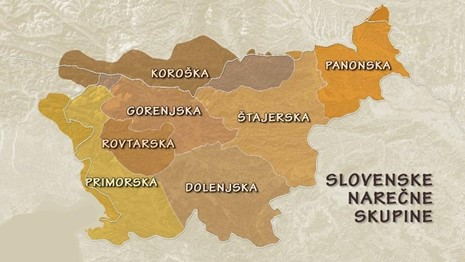
\includegraphics[width=1\linewidth]{narecne_skupine.jpg}
        \caption{Image 1: Slovene dialect groups
}
        \label{fig:map}
    \end{figure}

\subsection{2.1. Littoral Dialect Group}

    The Littoral dialect group comprises nine dialects: the Resian dialect (rezijansko narečje), the Torre Valley dialect (\textit{tersko narečje}), the Soča dialect (obsoško narečje}), the Natisone Valley dialect (\textit{nadiško narečje}), the Brda dialect (\textit{briško narečje}), the Karst dialect (\textit{kraško narečje}), the Istrian dialect (istrsko narečje}), the Čičarija dialect (\textit{čiško narečje}), and the Inner Carniolan dialect (\textit{notranjsko narečje}) (\cite{Novljan 2017}.)

\begin{figure}
    \centering
    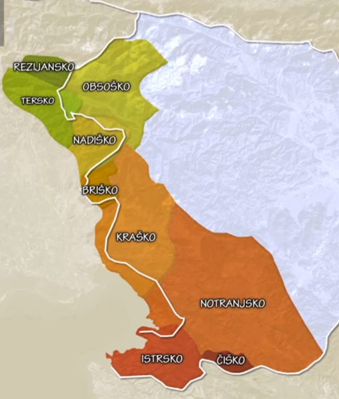
\includegraphics[width=0.5\linewidth]{Littoral.png}
    \caption{Image 2: Littoral dialect group
}
    \label{fig:map}
\end{figure}

\subsection{2.2. Styrian Dialect Group}

    The Styrian dialect group is spoken in the central and western parts of Slovenian Styria, in Maribor and its surroundings, in southern Pohorje, in lower and upper parts of Savinjska Valley, in Celje, Velenje, and the surrounding areas, as well as in Kozjansko and Bizeljsko. To the east, the Styrian dialect group extends to Slovenske Gorice and the lower course of the Drava river, gradually transitioning into the Panonian dialect group (\cite{Wikipedia 2023}).

    The Styrian dialect group is one of the seven main dialect groups in Slovenia and includes the following dialects: Central Savinja dialect (\textit{srednjesavinjsko narečje}), Upper Savinja dialect (\textit{zgornjesavinjsko narečje}) with Solčava sub-dialect (\textit{solčavsko podnarečje}), Central Styrian dialect (\textit{srednještajersko narečje}), Kozje-Bizeljsko dialect (\textit{kozjansko-bizeljsko narečje}), South Pohorje dialect (južnopohorsko narečje) with Kozjak subdialect (\textit{kozjaško podnarečje}), Lower Sava Valley dialect (\textit{posavsko narečje}) with Zagorje-Trbovlje subdialect (zagorsko-trboveljsko podnarečje), Laško subdialect (\textit{laško podnarečje}), and Sevnica-Krško subdialect (\textit{sevniško-krško podnarečje}) (\cite{Novljan 2017}). 
    
\begin{figure}
    \centering
    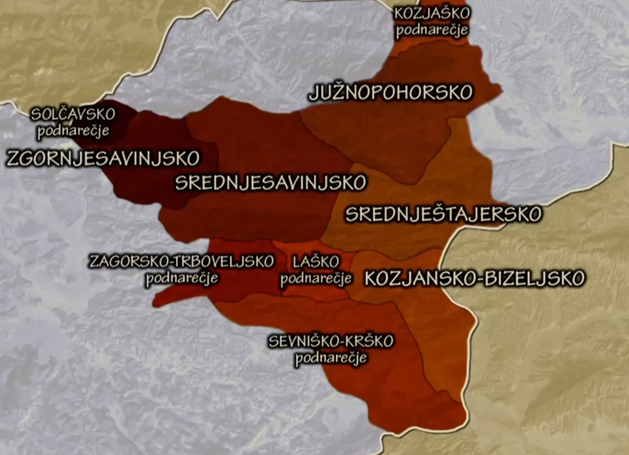
\includegraphics[width=1\linewidth]{styria.png}
    \caption{Image 4: Styrian dialect group
}
    \label{fig:map}
\end{figure}


    The Styrian dialect group also has some recognizable characteristics that distinguish it from other dialect groups: 

\begin{enumerate}
    \item The long stressed \textit{/e/} and falling \textit{/o/} developed into diphthongs \textit{/ei/} and \textit{/ou/}, while the old acute \textit{jat} was represented by the short narrow \textit{/e/}, and the new acute \textit{/o/} by the short \textit{/o/} (zvéizda, snéig, leis; mouč).

    \item The Upper Savinja dialect and Pohorje dialect are characterised by the lengthening of accented vowels, which is reflected in the double long representatives for \textit{/e/} and \textit{/o/} (zvâizda, snâik, pâič, brîza, nîsu in the Upper Savinja dialect and nusim, hudim in Pohorje dialect). 

    \item In some parts, the vowel \textit{/u/} changed to \textit{/ü/}, while in other parts remained the same or developed into \textit{/uu/} or \textit{/ou/}. The first change \textit{/ü/} is mainly found in the Central Styrian dialect. The vowel remained the same in the Central Savinja dialect and the Upper Savinja dialect. In the Pohorje dialect the vowel u developed into /\textit{uu/} or \textit{/ou/} (muha; müha; mu˛uha; mo˛uha).

    \item The long \textit{/a/} has been preserved in some parts of the Stryia territory, while in other parts it has been labiovelarized to a more or less wide \textit{/o/} (mačka; močka).

    \item The Styrian dialect does not distinguish between rising and falling accents in either long or short syllables. The tonal pattern in the Styrian dialect is mainly falling (\cite{Logar 1975}).
\end{enumerate}

%------------------------------------------------

\section{3. Methodology}

\subsection{3.1. Selection of LLMs}

    In the initial phase of our research, we evaluated the available Large Language Models (LLMs) that are suitable for our project's goal. After a thorough assessment, we decided to use the open-source language models Gemini and GPT-3.5. These selections were based on their demonstrated proficiency in understanding and modeling the Slovenian language.

    Within our methodology, we also examined alternative LLMs such as Llama 2 and Llama 3 to assess their suitability for replicating Slovenian dialects. However, it turned out that these models were insufficiently trained on Slovenian texts, which impaired their ability to successfully imitate the language, let alone its dialects.
    
\subsection{3.2. Prompts design}

    To ensure the accurate representation of Slovenian dialect nuances, we carefully created 25 prompts tailored to each dialect. These 50 prompts (25 for each dialect) were designed to incorporate dialect-specific vocabulary, grammatical structures, and cultural references, facilitating the understanding and reproduction of dialectal variations by the Large Language Models (LLMs). 
    
    To ensure robustness and generalisability of our results, we incorporated a wide range of topics and genres into our prompts. These prompts ranged from everyday conversations to technical discussions, literary extracts, and cultural and historical references, providing a diverse testing ground for the LLMs' dialectical reproduction abilities. By exposing the models to different linguistic contexts, we aimed to capture their performance in different fields and settings.
    
\subsection{3.3. Execution and response retrieval}

    After designing the prompts, we inputted them into the selected LLMs, comprising of Gemini and GPT-3.5, using their respective APIs or interfaces. Once the prompts were entered, we waited for the models' responses, which were autonomously generated  based on the provided instructions and the models' learnt patterns and language understanding capabilities.
    
\subsection{3.4. Data collection and analysis}

    After the prompts were executed, we systematically documented the responses generated by the LLMs in separate documents. Each document contained the LLM's responses to the prompts in the two different dialects, enabling the capture of nuanced linguistic variations produced by the models. This documentation process ensured the preservation and organisation of the response data for further analysis.

    For a comprehensive analysis, we created a separate set of documents for each LLM and each dialect. This approach allowed us to compare how well each specific model replicated dialects in general versus how the models in general replicated a specific dialect. By splitting the response data into separate sets of documents, we were able to isolate and evaluate the performance of each LLM across different dialectal variants more efficiently.

    With the document sets established, we conducted a comparative analysis to evaluate the accuracy of dialectal reproduction produced by each LLM. This analysis involved examining lexical choices, grammatical structures, idiomatic expressions, and cultural references within the generated responses. By comparing the responses between the different dialects and models, we were able to gain insights into the models' ability to reproduce dialectal nuances and their overall performance in dialect reproduction tasks.

\subsubsection{3.4.1. Natural Language Inference in assessing dialect adherence }

    To determine the Natural Language Inference (NLI) labels for the models' responses, we established a framework that evaluated the responses according to two main factors. Firstly, we checked whether the responses aligned with the provided context and genre given in the instructions. Secondly, we analysed whether the dialect use matched the given prompt. The criteria for assigning NLI labels based on dialect usage were as follows:

1. \textbf{Entailment}: This label is assigned when the dialect used in the response is consistent with the instructed dialect and reflects an authentic representation of the desired language style.

2. \textbf{Neutrality}: This label is assigned when the response contains elements of the instructed dialect, but occasionally also includes features of other dialects or standard Slovene. However, the predominant dialect remains consistent with the given instructions.

3 \textbf{Contradiction:} This label is assigned when another dialect is used in the answer and it differs from the given dialect, or when no dialect is used, which contradicts the given requirements.


%------------------------------------------------

\section*{4. Evaluation of LLMs}

    In this chapter, we will delineate a series of methodological challenges encountered while formulating prompts for Gemini and GPT-3.5.

\subsection*{4.1. Gemini}

    During our exploration of text generation with Gemini, we encountered a series of methodological challenges. Our analysis revealed that Gemini often produced more paragraphs than instructed, despite explicit directives to produce only two paragraphs. Furthermore, it frequently disregarded the instruction specifying that each paragraph should consist of a maximum of five sentences. Clarity regarding paragraph and sentence structure was in some examples achieved only when explicit instructions were provided - to generate precisely two paragraphs, each with a maximum of five sentences. Although the prompts did not explicitly call for the inclusion of a title and conclusion, Gemini, in most instances, produced titles for both the first and second paragraphs and concluded with a final thought on the text. 

    However, a more significant issue occurred when we attempted to generate dialect-specific content. Despite instructions to produce distinctly dialectal content, Gemini predominantly produced a text in standard Slovene. Despite additional prompts, Gemini still predominantly produced texts in standard Slovene and included numerous linguistic fillers (such as \textit{pač}), interjections (such as \textit{joj}), rhetorical figures (such as \textit{slikoviti griči}, \textit{ponosni stražarji}, and \textit{sonce na krožniku}), rhetorical questions (such as \textit{Družina, ja to je pa nekakšen temelj našega življenja, mar ne?}), and colloquial expressions (such as \textit{ful}, and \textit{faca}), rather than incorporating authentic dialectal expressions. It was only upon repeated prompts that Gemini exhibited some degree of dialectal authenticity, which was predominantly present in the first paragraphs of the texts.  

\subsection*{4.2. GPT-3.5}

While working with OpenAI’s large language model GPT-3.5, we noticed the following:

    Firstly the model adhered well to the context-based instructions regarding the topic of the text and its length. It never generated a response that was too short or long and it stuck to the instructed topic. 

    Secondly, the model often produced passages in standard Slovene (knjižna/standardna slovenščina). This most often occurred in the model’s first response to the prompt. It almost seemed as if the model ignored the instructions to write in the specified dialect (either the Štajersko or Notranjsko dialects). However, when another prompt followed with the instructions to once again “remind” the model to produce text that is not standard, GPT-3.5 managed to include regional and dialectal words, phrases, and other linguistic elements. 

An example of such behaviour is:

\textbf{Prompt}:
Napiši besedilo o tem, kako tehnologija vpliva na ljudi. Besedilo naj bo dolgo 2 odstavka, v prvem se osredotoči na vpliv po vsem svetu, v drugem pa na Slovenijo. Da bo bolj avtentično, ga napiši v izrazitem štajerskem narečju.

\textbf{Answer:}
\textit{Tehnologija je postala nepogrešljiv del našega vsakdana in vpliva na nas na mnogo načinov po vsem svetu. Z razvojem pametnih telefonov, računalnikov in družbenih omrežij smo postali bolj povezani in informirani kot kdajkoli prej. Vendar pa lahko pretirana uporaba tehnologije vodi v izolacijo, pomanjkanje fizične aktivnosti ter težave s spanjem in duševnim zdravjem. Poleg tega tehnološki napredki prinašajo tudi nove izzive, kot so varovanje zasebnosti, kibernetski napadi in odvisnost od digitalnih naprav.}

\textit{V Sloveniji pa je vpliv tehnologije podoben kot drugod po svetu. Pametni telefoni, računalniki in internet so postali nepogrešljiv del vsakdana tudi tukaj. Ljudje se povezujejo preko družbenih omrežij, opravljajo nakupovanje preko spleta in izvajajo delo na daljavo. Vendar pa je pomembno, da se zavedamo pasti pretirane uporabe tehnologije in da znamo najti ravnotežje med digitalnim svetom in resničnim življenjem. Spremljanje novih tehnoloških trendov je pomembno tudi za slovensko družbo, saj lahko tehnološki napredki prinašajo tako priložnosti kot tudi izzive.}

\textbf{Follow-up prompt:}
Besedilo napiši bolj narečno - v štajerskem narečju.

\textbf{Follow-up answer:}
\textit{Tehnologija je že postala del našega vsakdana pa vpliva na nas na mnogo načinov po vsem svetu. Z razvojem pametnih telefonov, računalnikov pa družbenih omrežij smo postali bolj povezani pa informirani kak kdajkoli prej. Ampak, preveč ziher uporabe tehnologije pa lahko pelje v izolacijo, manko fizične aktivnosti pa težave s spanjem pa duševnim zdravjem. Pa tudi tehnološki napredki prinesejo nove izzive, kak so varovanje zasebnosti, kibernetski napadi pa odvisnost od digitalnih stvari.}

\textit{V Sloveniji pa je vpliv tehnologije podoben, kak drugje po svetu. Pametni telefoni, računalniki pa internet so že postali del vsakdana tut tle. Ljudje se povezujejo preko družbenih omrežij, opravljajo nakupovanje preko spleta pa delajo od doma. Ampak, pomembno je, da se zavedamo pasti preveč uporabe tehnologije pa da znamo najti ravnotežje med digitalnim svetom pa realnim življenjem. Spremljanje novih tehnoloških trendov je tudi tuki pomembno, ker tehnološki napredki lahko prinesejo tako priložnosti pa tudi izzive za slovensko družbo.}

    After nudging the model to write more in-line with the mentioned dialect, one can also observe how it indeed wrote the passage with “strong” dialectal elements (in this case with words such as \textit{pa, kak, ziher, tut }etc.), but the way they fit into the text makes little sense to the native speaker of the dialect. Most of the passage is still in-line with standard Slovene and the regional nuances seem to be placed into the text at random. An example of this is the model keeping the standard word \textit{tudi }(‘also’) for most occurrences, but switching to its dialectal variant \textit{tut} only once. It would make “sense” for the model to switch either 100\% or 0\% of the time, but this was not the case.

    Another issue worth mentioning is how the model switched between dialects. When producing answers in a specific dialect, it often switched to another dialect at, what seemed, random. This can also be observed in the above example. The model used \textit{tle }and \textit{tuki} as variants of the standard Slovene \textit{tu/tukaj }(‘here’), but these words are not a part of the Styrian dialect, as they most commonly belong to the dialects found in more central Slovenia.



%------------------------------------------------

\section*{5. Results}

When analyzing the Styrian dialect (štajersko narečje) and Littoral dialect (notranjsko narečje), we noticed great disparities between the two models. Due to the apparent differences, we will present our findings for each model separately.

\subsection*{5.1. Littoral dialect}

\subsubsection{5.1.1. GPT-3.5}

    When considering the instructions regarding the length and the genre of the text, the GPT-3.5 model consistently adhered to the guidelines and did not exceed the limitations regarding paragraphs and the number of sentences per paragraph. The generated paragraphs within texts were clearly connected, with paragraphs complementing each other, thus ensuring that all generated texts maintained a logical coherence. 

    Regarding adherence to instructions for generating text in Littoral dialect (notranjsko narečje), GPT-3.5 was not as successful. Following the initial instructions, it predominantly produced texts in standard Slovene (standardna/knjižna slovenščina). After additional prompts and instructions, it yielded improved results, yet the texts still remained rich with expressions in standard Slovene. In some instances, it utilized expressions from the Lower Caroniolan dialect (such as \textit{tut}, \textit{važn}, \textit{dost} etc.) and incorporated numerous colloquial and slang expressions (such as \textit{ful}, \textit{fora}, \textit{fajn}, \textit{folk} etc.). In some texts it still produced some distinctly Littoral dialect expressions (such as \textit{kanta}, \textit{spoštavajo}, \textit{našga}, \textit{proba}, \textit{pr}', \textit{en caj}t etc.). However, at times, despite the instruction to write the text in the Littoral dialect, it incorporated expressions from other dialectal groups (such as \textit{kak}, \textit{tut}, \textit{ka} etc).

\subsubsection{5.2.2. Gemini}

    In terms of adhering to the content and genre instructions, Gemini performed equally well as the GPT-3.5 model. However, regarding the length of the text, Gemini in most cases exceeded the specified limitations. It added more paragraphs, with paragraphs being longer than the specified limit, and frequently provided a conclusion at the end of the text. Another distinction is that Gemini generated titles for each paragraph, even though this was not specified in the instructions. 

    In generating text in distinctive Littoral dialect (notranjsko narečje), Gemini's performance was inferior to that of GPT-3.5. Initially, similar as GPT-3.5, it produced predominantly standard Slovene texts. However, with additional prompts and instructions, it gradually incorporated some Litteral dialect expressions (such as \textit{inu}, \textit{finte}, \textit{proba}, \textit{fešta}, \textit{bejž'te}, \textit{pr' }etc.). Throughout, it used numerous linguistic fillers (such as \textit{pač}, \textit{pa} etc.). Similarly to GPT-3.5, it utilized a lot of colloquial and slang terms (such as \textit{fajn}, \textit{faca}, \textit{fora} etc.). Unlike GPT-3.5, Gemini also incorporated some rhetorical figures (such as \textit{sonce na krožniku}, \textit{slikoviti griči} etc.) and some diminutives (like \textit{mestece}, \textit{cvičkotom} etc.). An important observation is that in the first paragraph generated more Littoral  dialectal expressions compared to the second paragraph. 
    
\subsection{5.2. Styrian dialect}

\subsubsection{5.2.1. GPT-3.5}

    When it comes to context and genre, GPT-3.5 followed the requested topics 100\% of the time, being assigned the entailment label in all cases. It clearly had no trouble writing an answer that was contextually in-line with the prompt.

    However, it did not perform as well in regards to the dialect criteria. While it adhered to the Styrian dialect some of the time, its answers were most frequently classified as neutral. This is due to the fact that while it often produced some dialectal words and patterns, it also included some words from other dialects and/or in standard Slovene. It never received a contradiction label, as there was no case where it did not use at least some words in the specified dialect. 

    Another observation is the fact that, as mentioned above, it often did not produce a dialectal text from the first prompt. We sometimes had to give it a follow-up prompt in order for it to produce an answer that was not written in standard Slovene.

\subsubsection{5.2.2. Gemini}

    Context- and genre-wise, Gemini performed just as well as GPT-3.5, scoring the entailment tag in 100\% of the cases. Like GPT-3.5, the model had no issues with generating text that followed the topic provided in the instructions.

    When it comes to dialects, however, the results were much worse than GPT-3.5. It failed to receive a single entailment tag. This is mostly due to the facts mentioned above, namely that it almost always produced text in standard Slovene. It sometimes began the excerpt with a single sentence that contained a few Styrian dialectal words, but then went on to write everything else in standard Slovene.

%------------------------------------------------

\section*{6. Discussion}

\subsection{6.1. Possible solutions}

    When analyzing the produced texts and our prompts, we came up with a few solutions that could help the models get better scores according to NLI tagging. We present the solutions in the following subsections.

\subsubsection{6.1.1 Follow-up prompts with dialect emphasis}

    An effective solution we implemented to improve the accuracy of dialectal reproduction by the LLMs was the use of follow-up prompts emphasising the use of the target dialect. After receiving the initial responses from the language models, we developed follow-up prompts that reiterated the previous instructions while explicitly emphasising the specific dialect that the model was to reproduce. By reinforcing the dialect and providing clear instructions, these follow-up prompts served to guide the LLMs towards more accurate and authentic dialectal responses.

An example of this can be observed in the following prompt that was conducted on GPT-3.5:

\textbf{Prompt}: 
Napiši besedilo dolgo 2 odstavka. Vsak odstavek naj ima približno pet povedi. V prvem odstavku piši o slovenski glasbi, v drugem odstavku pa se osredotoči na slovensko ljudsko glasbo. Da bo besedilo bolj avtentično, ga napiši v izrazitem notranjskem narečju.

\textbf{Answer:}
\textit{Slovenska glasba ima dolgo in pestro zgodovino. Naša glasbena dediščina sega vse od ljudskih pesmi, ki so jih prepevali naši predniki, do sodobnih glasbenih žanrov, ki jih ustvarjajo sodobni slovenski glasbeniki. Imamo raznolike žanre, kot so ljudska glasba, pop, rock, rap, jazz in še mnogi drugi, ki bogatijo glasbeno krajino Slovenije. Slovenski glasbeniki so dosegli številne uspehe tako doma kot v tujini, kar je prispevalo k prepoznavnosti naše glasbene scene po celem svetu. Glasba je pomemben del našega kulturnega izraza in identitete ter ima moč, da združuje ljudi ne glede na njihovo poreklo in prepričanja.}

\textit{Ljudska glasba pa ima posebno mesto v slovenskem srcu. To je glasba, ki je prenašana iz roda v rod in je zapisana v dušo našega naroda. Ljudske pesmi so pogosto povezane z različnimi prazniki, običaji in življenjskimi dogodki ter odražajo bogato kulturno dediščino Slovenije. Njihovi ritmi in melodije so preprosti, a hkrati ganljivi in močno čustveni, kar nas povezuje s preteklostjo in nas navdaja z občutkom pripadnosti. Ljudska glasba se še danes ohranja in neguje v številnih folklornih skupinah ter prireditvah po vsej Sloveniji, kar kaže na pomembnost in trajnost te dragocene glasbene tradicije.}

\textbf{Folow-up prompt:} 
Besedilo napiši bolj narečno - v notranjskem narečju.

\textbf{Follow-up answer:}
\textit{Slovenska muzka ma pr' nas dolgo in pestró zgodovino. Naša muzikalna dediščina seže vse od ljudskih štosev, ki so jih pel naši stari fotri, do današnjih modernih zvrsti, ki jih glasbeniki ustvarjajo. Mamo raznolike zvrsti, kot so ljudska muzka, pop, rock, rap, jazz in še mnogo drugih, k se pač delajo muziko pri nas. Slovenski muzikanti so dosegl že mnoge uspehe tako doma kot v tujini, kar je pač prinesl, da nas poznajo širom sveta. Muzka je pač pomemben del našega kulturnega izraza in identitete ter majo moč, da združujejo ljudi, ne glede na to, kje so in kaj so.}

\textit{Ljudska muzka pa ma res posebno mesto pr' nas. To je muzka, ki se prenaša iz roda v rod in je zapisana v dušo našga naroda. Ljudske pesmi so pač povezane z različnimi prazniki, običaji in življenjskimi dogodki ter odražajo bogato kulturno dediščino Slovenije. Njihovi ritmi in melodije so pač preprosti, ampak hkrati ganljivi in močno čustveni, kar nas pač povezuje s preteklostjo in nas polni s tem občutkom pripadnosti. Ljudska muzka se še danes ohranja in neguje v številnih folklornih skupinah ter prireditvah po vsej Sloveniji, kar kaže na pomembnost in trajnost te dragocene muzikalne tradicije.}

\subsubsection{6.1.2 Focus on the dialect of a specific region
}
\subsubsection{6.1.3 More precise and clear instructions
}
\subsubsection{6.1.4 Compilation of a glossary for the Styrian and Littoral dialects
}
\subsubsection{6.1.5 Use of the Poun Kufr online dictionary for the Inner Carniolan dialect
}
\subsubsection{6.1.6 Consideration of phonology and marking emphasis}

\subsubsection{6.1.7 Separate instructions tailored specifically to one LLM}

%------------------------------------------------

\section*{Acknowledgments}



%----------------------------------------------------------------------------------------
%	REFERENCE LIST
%----------------------------------------------------------------------------------------

    Inštitut za slovenski jezik Frana Ramovša ZRC SAZU and Geografski inštitut Antona Melika ZRC SAZU and Inštitut za antropološke in prostorske študije ZRC SAZU. “Karta slovenskih narečij z večjimi naselji”. 2016. \href{https://fran.si/204/sla-slovenski-lingvisticni-atlas/datoteke/SLA_Karta-narecij.pdf}{https://fran.si/204/sla-slovenski-lingvisticni-atlas/datoteke/SLA\_Karta-narecij.pdf}

    Logar, Tine. \textit{Slovenska Narečja: Besedila}. Ljubljana: Mladinska knjiga, 1975.

    Novljan, Neva, Barbara Ivančič Kutin, Klara Šumenjak, and Karin Marc Bratina. 2017. “Slovenska narečja, Primorska narečna skupina”. Ljubljana: Radiotelevizija Slovenija javni zavod. 2017. \href{https://365.rtvslo.si/arhiv/dokumentarni-filmi-in-oddaje-kulturno-umetniski-program/174451674}{https://365.rtvslo.si/arhiv/dokumentarni-filmi-in-oddaje-kulturno-umetniski-program/174451674}. 

    Novljan, Neva, Tjaša Jakop, and Peter Weiss. 2017. “Slovenska narečja, Štajerska narečna skupina”. Ljubljana: Radiotelevizija Slovenija javni zavod. 2017. \href{https://365.rtvslo.si/arhiv/dokumentarni-filmi-in-oddaje-kulturno-umetniski-program/174453174}{https://365.rtvslo.si/arhiv/dokumentarni-filmi-in-oddaje-kulturno-umetniski-program/174453174}.

    Pahor, M., N. Pahor, R. Pahor, and B. P. Arčon. \textit{Po Ríenškuo: Muója Besíeda Je Múej Dúem : [Renške Narečne Besede : Prispevki Za Slovar]}. Društvo za kulturo, turizem in razvoj, 2016.

    “Štajerska Narečna Skupina.” Wikipedia, August 13, 2023. \href{https://sl.wikipedia.org/wiki/\%C5\%A0tajerska_nare\%C4\%8Dna_skupina}{https://sl.wikipedia.org/wiki/\%C5\%A0tajerska\_nare\%C4\%8Dna\_skupina}. 


\end{document}